\section{Navegação Reativa em Robótica Móvel}

A navegação é uma capacidade fundamental para robôs móveis autônomos, permitindo que se desloquem de forma segura e eficiente em ambientes diversos. Esta seção apresenta os principais paradigmas de navegação robótica, com ênfase na navegação reativa, particularmente relevante para aplicações em ambientes dinâmicos e não estruturados como subestações elétricas.

\subsection{Paradigmas de Navegação Robótica}
A \autoref{fig:paradigmas_navegacao} mostra como a navegação robótica pode ser classificada em diferentes paradigmas, cada um com abordagens distintas para o problema de deslocamento autônomo \cite{Siegwart2011, Murphy2000}.

\begin{figure}[h]
    \centering
%% Figura refeita em 14/11/2026. A versao anterior estava errada e era redundante: a
%% coluna "Hibrida" trazia TRES caixas "Act" e NENHUMA "Plan", apagando o planejamento
%% justo onde ele define o conceito; os rotulos estavam em ingles; e o desenho repetia
%% a tricotomia da Figura~\ref{fig:arquiteturas_roboticas}, a uma secao de distancia.
%% A versao atual mostra o que e especifico de NAVEGACAO -- a mesma planta com os
%% mesmos obstaculos, variando o tracado --, de modo que as duas figuras deixam de se
%% sobrepor.
    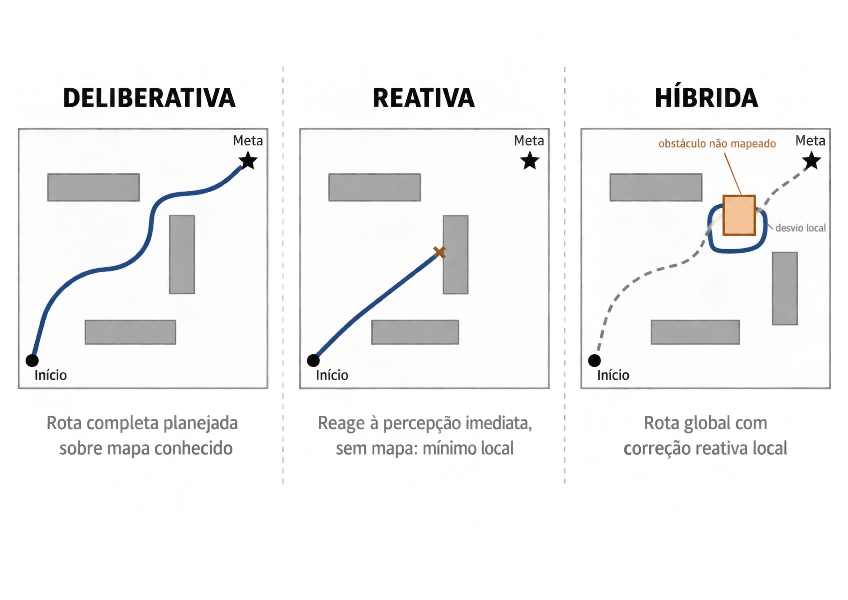
\includegraphics[width=0.8\textwidth]{figuras/fig_paradigmas_navegacao.pdf}
    \caption{Paradigmas de navegação robótica sobre a mesma planta: à esquerda, a rota
    completa planejada sobre mapa conhecido; ao centro, a reação à percepção imediata,
    que sem mapa fica retida num mínimo local antes de alcançar a meta; à direita, a
    rota global corrigida localmente ao encontrar um obstáculo não mapeado.}
    \legend{Fonte: Adaptado de \citeonline{Siegwart2011} e \citeonline{Murphy2000}.}
    \label{fig:paradigmas_navegacao}
\end{figure}


\subsubsection{Navegação Deliberativa}

A navegação deliberativa segue o paradigma Sense-Plan-Act (SPA), onde o robô percebe o ambiente, constrói um modelo interno, planeja uma trajetória completa e então a executa \cite{Murphy2000}. Suas principais características incluem:

\begin{itemize}
    \item Representação explícita do ambiente através de mapas detalhados
    \item Planejamento global de trajetórias completas
    \item Busca por soluções ótimas segundo critérios específicos
    \item Maior complexidade computacional
    \item Sensibilidade a incertezas e discrepâncias no modelo do ambiente
\end{itemize}

\subsubsection{Navegação Reativa}

Em contraste, a navegação reativa baseia-se no paradigma Sense-Act, eliminando a fase explícita de planejamento \cite{Brooks1986, Arkin1998}. O robô reage diretamente aos estímulos sensoriais, sem construir um modelo completo do ambiente. Suas características incluem:

\begin{itemize}
    \item Ausência de representação explícita do ambiente
    \item Decisões baseadas apenas na percepção imediata
    \item Baixa complexidade computacional
    \item Robustez a incertezas e mudanças no ambiente
    \item Possibilidade de soluções subótimas ou mínimos locais
\end{itemize}

\subsubsection{Navegação Híbrida}

A navegação híbrida combina elementos das abordagens deliberativa e reativa \cite{Murphy2000, Arkin1998}, tipicamente organizados em camadas:

\begin{itemize}
    \item Camada deliberativa para planejamento global e raciocínio de alto nível
    \item Camada reativa para respostas rápidas a eventos imprevistos
    \item Camada intermediária para coordenação entre as demais
\end{itemize}

Exemplos incluem a arquitetura 3T \cite{Bonasso1997}, AuRA \cite{Arkin1987} e Saphira \cite{Konolige1997}.

\subsection{Navegação Baseada em Comportamentos}

A navegação baseada em comportamentos é uma abordagem reativa que organiza o controle do robô em módulos comportamentais simples e independentes \cite{Arkin1998, Brooks1986}.

\subsubsection{Arquitetura de Subsunção}

A Arquitetura de Subsunção, proposta por Rodney Brooks \cite{Brooks1986}, organiza os comportamentos em camadas hierárquicas, onde comportamentos de nível superior podem suprimir ou inibir comportamentos de nível inferior. Suas características incluem:

\begin{itemize}
    \item Decomposição vertical em níveis de competência
    \item Incrementalidade na construção do sistema
    \item Mecanismos de supressão e inibição para coordenação
    \item Ausência de representação central do ambiente
\end{itemize}

Uma implementação típica inclui comportamentos como evitar obstáculos (nível básico), vagar, explorar, construir mapas e identificar objetos (níveis superiores) \cite{Brooks1986}.

\subsubsection{Esquemas Motores}

A abordagem de Esquemas Motores, proposta por Ronald Arkin \cite{Arkin1989}, utiliza fusão de comportamentos através de soma vetorial. Suas características incluem:

\begin{itemize}
    \item Representação vetorial de cada comportamento
    \item Fusão por soma ponderada dos vetores
    \item Pesos adaptativos para os comportamentos
    \item Paralelismo na contribuição dos comportamentos
\end{itemize}

A equação básica para a fusão de comportamentos é:

\begin{equation}
\vec{v} = \sum_{i=1}^{n} w_i \cdot \vec{v_i}
\end{equation}

onde $\vec{v}$ é o vetor resultante, $\vec{v_i}$ é o vetor gerado pelo comportamento $i$, $w_i$ é o peso associado ao comportamento $i$, e $n$ é o número total de comportamentos \cite{Arkin1998}.

\subsection{Campos Potenciais e Navegação Reativa}

O método de Campos Potenciais, introduzido por Oussama Khatib \cite{Khatib1986}, representa o ambiente como um campo de forças, onde o robô é atraído pelo objetivo e repelido por obstáculos.

\subsubsection{Princípios Fundamentais}

No método de Campos Potenciais, o robô é tratado como uma partícula sob influência de um campo potencial artificial $U(q)$, que é a soma de um potencial atrativo $U_{att}(q)$ gerado pelo objetivo e potenciais repulsivos $U_{rep}(q)$ gerados pelos obstáculos \cite{Khatib1986, Siegwart2011}:

\begin{equation}
U(q) = U_{att}(q) + U_{rep}(q)
\end{equation}

A força resultante que atua sobre o robô é o gradiente negativo do potencial total:

\begin{equation}
F(q) = -\nabla U(q) = -\nabla U_{att}(q) - \nabla U_{rep}(q) = F_{att}(q) + F_{rep}(q)
\end{equation}

O potencial atrativo é tipicamente definido como uma função quadrática da distância ao objetivo:

\begin{equation}
U_{att}(q) = \frac{1}{2} \xi \|q - q_{goal}\|^2
\end{equation}

O potencial repulsivo cresce à medida que o robô se aproxima de obstáculos:

\begin{equation}
U_{rep}(q) = 
\begin{cases}
\frac{1}{2} \eta \left(\frac{1}{\rho(q)} - \frac{1}{\rho_0}\right)^2, & \text{se } \rho(q) \leq \rho_0 \\
0, & \text{se } \rho(q) > \rho_0
\end{cases}
\end{equation}

onde $\eta$ é um fator de escala, $\rho(q)$ é a distância ao obstáculo mais próximo e $\rho_0$ é a distância de influência do obstáculo \cite{Khatib1986, Siegwart2011}.

\subsubsection{Limitações e Extensões}

Apesar de sua simplicidade e eficiência computacional, o método de Campos Potenciais apresenta algumas limitações \cite{Koren1991, Siegwart2011}:

\begin{itemize}
    \item Mínimos locais que podem "aprisionar" o robô
    \item Oscilações em passagens estreitas
    \item Dificuldades quando o objetivo está próximo a obstáculos
    \item Falta de consideração da dinâmica do robô
\end{itemize}

Diversas extensões foram propostas para superar estas limitações, incluindo Campos Potenciais Harmônicos \cite{Connolly1990}, combinação com navegação em grafo \cite{Barraquand1992}, e abordagens evolutivas \cite{Vadakkepat2000}.

\subsubsection{Aplicações em Robótica Móvel}

O método de Campos Potenciais tem sido aplicado com sucesso em diversas áreas \cite{Siegwart2011, Arkin1998}:

\begin{itemize}
    \item Robôs móveis terrestres para navegação em ambientes internos e externos
    \item Veículos aéreos não tripulados para navegação 3D
    \item Robôs manipuladores para planejamento de movimento
    \item Sistemas multi-robôs para coordenação de enxames
\end{itemize}

Em aplicações de inspeção de subestações elétricas, a navegação reativa baseada em campos potenciais oferece vantagens significativas devido à sua capacidade de responder rapidamente a obstáculos imprevistos e adaptar-se a ambientes dinâmicos \cite{Lactec2022, Iberdrola2022}.

\subsection{SLAM (Simultaneous Localization and Mapping)}

O SLAM é um problema fundamental em robótica móvel que consiste em construir um mapa do ambiente desconhecido enquanto simultaneamente se localiza neste mapa \cite{Durrant2006, Thrun2005}.

\subsubsection{O Problema do SLAM}
Os principais desafios do SLAM incluem incertezas na odometria e nas medições, associação de dados, alta dimensionalidade do espaço de estados e ambiguidade perceptual \cite{Durrant2006, Thrun2005}. A \autoref{fig:problema_slam} mostra uma visão geral do uso do SLAM na navegação.

\begin{figure}[h]
    \centering
%% Figura refeita em 14/11/2026. A versao anterior nao mostrava o problema: exibia
%% quatro setas soltas entre robo, ambiente e mapa, sem a circularidade que e a
%% dificuldade inteira do SLAM. Equiparava ainda "comandos de controle" e "odometria"
%% num unico rotulo, sendo que u sao os comandos e a odometria e a medida do
%% deslocamento resultante, com incerteza propria.
    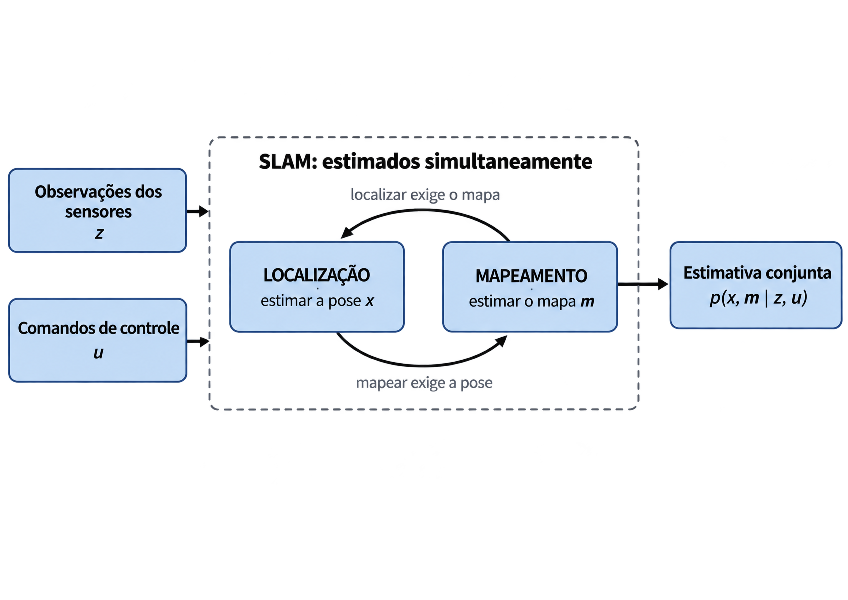
\includegraphics[width=0.8\textwidth]{figuras/fig_problema_slam.pdf}
    \caption{O problema do SLAM: localizar exige o mapa e mapear exige a pose, de modo
    que as duas estimativas são mutuamente dependentes e precisam ser resolvidas
    simultaneamente, a partir das observações $z$ e dos comandos de controle $u$.}
    \legend{Fonte: Adaptado de \citeonline{Durrant2006} e \citeonline{Thrun2005}.}
    \label{fig:problema_slam}
\end{figure}

O problema do SLAM pode ser formulado probabilisticamente como a estimação da distribuição de probabilidade conjunta \cite{Durrant2006, Thrun2005}:

\begin{equation}
p(x_{1:t}, m | z_{1:t}, u_{1:t}, x_0)
\end{equation}

onde $x_{1:t}$ são os estados do robô, $m$ é o mapa do ambiente, $z_{1:t}$ são as observações sensoriais, $u_{1:t}$ são os comandos de controle, e $x_0$ é o estado inicial.


\subsubsection{Principais Abordagens}

Diversas abordagens foram desenvolvidas para resolver o problema do SLAM \cite{Durrant2006, Thrun2005, Cadena2016}:

\begin{itemize}
    \item \textbf{SLAM Baseado em Filtros}: Utiliza técnicas como EKF-SLAM (Extended Kalman Filter) \cite{Smith1990}, UKF-SLAM (Unscented Kalman Filter) \cite{Julier2004} e FastSLAM (filtros de partículas) \cite{Montemerlo2002}.
    
    \item \textbf{SLAM Baseado em Otimização}: Formula o problema como minimização de erro, incluindo Graph-SLAM \cite{Grisetti2010} e Pose Graph Optimization.
    
    \item \textbf{SLAM Visual}: Utiliza câmeras como principal sensor, incluindo MonoSLAM \cite{Davison2007}, Stereo SLAM \cite{Paz2008} e Visual-Inertial SLAM \cite{Mourikis2007}.
    
    \item \textbf{SLAM Baseado em LiDAR}: Utiliza sensores laser, incluindo Hector SLAM \cite{Kohlbrecher2011}, Cartographer \cite{Hess2016} e LOAM \cite{Zhang2014}.
\end{itemize}

\subsubsection{Representações de Mapas}

Diferentes representações de mapas são utilizadas em SLAM \cite{Thrun2005, Cadena2016}:

\begin{itemize}
    \item Mapas de Ocupação em Grade (discretização do espaço em células) \cite{Elfes1989}
    \item Mapas de Características (pontos, linhas ou cantos distintos) \cite{Smith1990}
    \item Mapas Topológicos (grafo de locais e conexões) \cite{Kuipers1991}
    \item Mapas Semânticos (com informações sobre objetos e regiões) \cite{Kostavelis2015}
    \item Mapas 3D (nuvens de pontos, malhas ou octrees) \cite{Hornung2013}
\end{itemize}

O fechamento de loop (reconhecer quando o robô retorna a um local visitado) é o que corrige a deriva acumulada na odometria: detectado o reencontro, mapa e trajetória estimada são reajustados \cite{Durrant2006, Cadena2016}.

\subsection{Integração de Modelos 3D em Navegação}

A integração de modelos 3D em sistemas de navegação robótica representa uma tendência importante, especialmente para aplicações em ambientes complexos como subestações elétricas \cite{Hornung2013, Rusu2011}.

\subsubsection{Representações 3D para Navegação}

Diversas representações 3D são utilizadas para navegação robótica \cite{Hornung2013, Rusu2011}:

\begin{itemize}
    \item \textbf{Nuvens de Pontos}: Conjuntos de pontos 3D obtidos de sensores como LiDAR ou câmeras de profundidade.
    
    \item \textbf{Octrees}: Estruturas hierárquicas que dividem o espaço 3D recursivamente, como o OctoMap \cite{Hornung2013}.
    
    \item \textbf{Malhas Poligonais}: Representações de superfícies através de polígonos conectados.
    
    \item \textbf{Mapas de Elevação}: Representações 2.5D que armazenam a altura do terreno para cada posição (x,y).
\end{itemize}

\subsubsection{Aquisição e Processamento de Dados 3D}

A aquisição de dados 3D para navegação pode ser realizada através de \cite{Rusu2011, Hornung2013}:

\begin{itemize}
    \item Sensores LiDAR 3D ou 2D com movimento
    \item Câmeras RGB-D (como Kinect ou RealSense)
    \item Sistemas de visão estéreo
    \item Fotogrametria e Structure from Motion
\end{itemize}

O processamento destes dados envolve técnicas como registro de nuvens de pontos, filtragem, segmentação, detecção de características e reconstrução de superfícies \cite{Rusu2011}.

\subsubsection{Aplicações em Subestações Elétricas}

A integração de modelos 3D em navegação robótica para inspeção de subestações elétricas oferece diversas vantagens \cite{Lactec2022, Iberdrola2022}:

\begin{itemize}
    \item \textbf{Planejamento de Trajetória 3D}: Permite considerar a estrutura vertical das subestações, incluindo equipamentos elevados e obstáculos em diferentes alturas.
    
    \item \textbf{Localização Precisa}: Melhora a precisão da localização do robô através da correspondência com modelos 3D detalhados.
    
    \item \textbf{Detecção de Mudanças}: Permite identificar alterações na estrutura da subestação através da comparação com modelos de referência.
    
    \item \textbf{Inspeção Baseada em Modelos}: Facilita a inspeção direcionada de componentes específicos, utilizando o modelo 3D como referência.
    
    \item \textbf{Visualização e Análise}: Melhora a visualização e análise dos dados de inspeção no contexto do modelo 3D da subestação.
\end{itemize}

\subsection{Desafios e Tendências}

A navegação reativa em robótica móvel, especialmente para aplicações em subestações elétricas, enfrenta diversos desafios e apresenta tendências emergentes \cite{Cadena2016, Lactec2022, Iberdrola2022}.

\subsubsection{Desafios Atuais}

\begin{itemize}
    \item \textbf{Robustez a Interferência Eletromagnética}: Garantir o funcionamento adequado dos sensores e algoritmos de navegação em ambientes com forte interferência eletromagnética.
    
    \item \textbf{Navegação em Ambientes Complexos}: Lidar com a complexidade estrutural das subestações, incluindo equipamentos de diferentes formas e tamanhos, cabos, estruturas elevadas, etc.
    
    \item \textbf{Adaptação a Condições Variáveis}: Adaptar-se a mudanças nas condições ambientais, como iluminação, clima e configuração da subestação.
    
    \item \textbf{Segurança}: Garantir a navegação segura em ambientes de alta tensão, evitando colisões com equipamentos críticos e mantendo distâncias de segurança.
\end{itemize}

\subsubsection{Tendências Emergentes}

\begin{itemize}
    \item \textbf{Navegação Semântica}: Incorporação de informações semânticas no processo de navegação, permitindo decisões baseadas no significado e função dos objetos no ambiente.
    
    \item \textbf{Aprendizado de Navegação}: Utilização de técnicas de aprendizado de máquina para melhorar o desempenho da navegação através da experiência.
    
    \item \textbf{Navegação Colaborativa}: Coordenação entre múltiplos robôs para inspeção e navegação mais eficientes.
    
    \item \textbf{Integração com Digital Twins}: Utilização de modelos digitais detalhados das subestações para melhorar o planejamento e execução da navegação.
\end{itemize}

A navegação reativa em robótica móvel, especialmente quando integrada com técnicas de SLAM e modelos 3D, oferece uma base sólida para o desenvolvimento de sistemas robóticos autônomos capazes de realizar inspeções eficientes e seguras em subestações elétricas, contribuindo para a manutenção preventiva e a confiabilidade do sistema elétrico.
